\documentclass[letterpaper,12pt]{article}
\usepackage{tabularx} % extra features for tabular environment
\usepackage{amsmath}  % improve math presentation
\usepackage{graphicx} % takes care of graphic including machinery
\usepackage[margin=1in,letterpaper]{geometry} % decreases margins
\usepackage{cite} % takes care of citations
\usepackage[final]{hyperref} % adds hyper links inside the generated pdf file
\hypersetup{
	colorlinks=true,       % false: boxed links; true: colored links
	linkcolor=blue,        % color of internal links
	citecolor=blue,        % color of links to bibliography
	filecolor=magenta,     % color of file links
	urlcolor=blue         
}
\usepackage{blindtext}
%++++++++++++++++++++++++++++++++++++++++


\begin{document}

\title{Naive Bayes Classifier}
\author{Anshumaan Singh 18BCE2193}
\date{\today}
\maketitle

\begin{abstract}
In this assignment paper I studied the concept of Naive Bayes Classifiers which are a family of simple "probabilistic classifiers" based on applying Bayes' theorem with strong independence assumptions between the features. They are among the simplest Bayesian network models.   
\end{abstract}


\section{Introduction}

Naive Bayes is a subset of Bayesian choice hypothesis. It's called Naive on the grounds that the detailing makes some gullible 
presumptions. Python's content preparing capacities which split up a record into a vector are utilized. This can be utilized to characterize text. Characterizes may place into intelligible structure. It is a mainstream grouping technique notwithstanding restrictive freedom, over fitting, and Bayesian strategies. 
Notwithstanding the straightforwardness of Naive Bayes, it can characterize archives shockingly well. Instinctually a potential 
avocation for the contingent freedom supposition that will be that if the archive is about governmental issues, this is a decent proof of the sorts of different words found in the report. Innocent Bayes is a sensible classifier in this sense and has negligible capacity 
what's more, quick preparing, it is applied totime-stockpiling basic applications, for example, naturally ordering website pages into types and spam sifting. Thinking about a lot of articles, every one of which has a place with a known class, and every one of which has a known vector of factors, the point is to make a standard which empowers to allot future items to a class, given only the vectors of factors checking out the future items. These issues are known as ―supervised grouping problem‖, are around the world, and the greater part of the strategies for building such guidelines have been created. It is anything but difficult to set up, and no need any muddled monotonous boundary assessment plans. This implies it ought to be applied to gigantic informational collections. It is anything but difficult to decipher, so incompetent clients in 
classifier innovation can make out the purpose behind it is making the arrangement it makes. At last, it regularly does shockingly 
well: it ought not be the most ideal classifier in a specific application, however it can generally be depended on to be strong and to progress admirably.

\section{Naive Bayes Classifier}

A naïve Bayes classifier corresponds to a Bayesian network, as in Eq (1). Here, a single class variable C and m attribute variables Xi(for simplicity of exposition, attributesare discrete). Let c denote a class label and xi denote a value of an attribute Xi. A naïve Bayes induces a distribution:
Where we have a class prior Pr(C) and conditional distributions Pr(Xi|C). We can estimate these parameters from(labeled) data, using maximum likelihood or MAP estimation.Once we have learned a naïve Bayes classifier from data,we can label new instances by selecting the class label c* that has maximum posterior probability given observation sx1,...,xm. select:

\begin{figure}[!h]
    \centering
    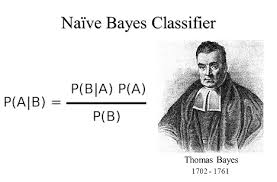
\includegraphics[width=.8\textwidth]{images.jpg}
    \caption{Naive Bayes is a subset of Bayesian choice hypothesis. It's called Naive on the grounds that the detailing makes some gullible 
presumptions.}
\end{figure}


\section{Augmented Naive Bayes}

Classification is a fundamental issue in machine learning and data mining. In classification, the goal of a learning
algorithm is to construct a classifier given a set of training examples with class labels. Regularlyexample E is represented by attribute values by a tuple(x1,x2, · · ·,xn), where xi is the value of attribute Xi. Let C represent the classification variable, and let c be the value of C. There are only two classes here: +(the positive class) or −(the negative class). A classifier is a function that assigns a class label to an example. From the probability perspective, according to Bayes Rule, the probability of an example E=(x1,x2,· · ·,xn) being class c is:
Innocent Bayes is the least complex type of Bayesian organization, wherein all credits are autonomous given the estimation of the class variable. This is called contingent freedom. Obviously the contingent freedom supposition that is rarely right in the vast majority of this present reality applications. A direct way to deal with control the constraint of credulous Bayes is to build its structure to speak to unequivocally the conditions among credits. An increased credulous Bayesian organization, or essentially enlarged guileless Bayes (ANB), is an all-encompassing innocent Bayes, that the class hub focuses to all ascribe hubs straightforwardly, and there discovered connections among property hubs. Figure 2 shows a case of ANB. From the perspective on plausibility, an ANB G shows a joint likelihood circulation portrayed underneath.

\begin{figure}[!h]
    \centering
    \includegraphics[width=.8\textwidth]{download (6).png}
    \caption{Tree augmented naive Bayes is a semi-naive Bayesian Learning method. It relaxes the naive Bayes attribute independence assumption by employing a tree structure, in which each attribute only depends on the class and one other attribute.}
\end{figure}


\section{Literature Survey}

In the paper [1], the current improved calculations are summed up and a novel Bayes model is proposed: Hidden Naive Bayes (HNB). In HNB, a shrouded parent is made for each characteristic which consolidates the impacts from every single other trait.A precise test concentrate on the grouping, class likelihood assessment and positioning execution of HNB is finished.The exploratory outcomes show that HNB has a superior generally execution contrasted with the other best in class models for increasing gullible Bayes.The structure of HNB contains one shrouded layer. It very well may be relied upon to stretch out to more perplexing structures, for example, twofold layers. This will be another subject for future examination.Innocent Bayes is among the least difficult probabilistic classifiers [2]. It frequently shows incredibly well in some genuine world applications, notwithstanding the solid suspicion that all highlights are temporarily free given the class. The estimations of these factors are found by tackling the likening streamlining issues. The acquired outcomes indicate that the proposed models can critically improve the presentation of the innocent Bayes classifier, yet simultaneously moderate its straightforward structure. This paper [2] has introduced three diverse advancement models for the innocent Bayes classifier. At that point applied improvement methods to locate the ideal qualities for these factors. Likewise, contrasted the proposed models and NB, TAN, the SVM, C4.5, and 1-NN on 14 genuine parallel arrangement informational collections. The estimations of highlights in informational indexes are individualized by utilizing a middle based individualization technique and applying two diverse individualization calculations, the Fayyad and Irani strategy and the calculation SOAC. Creators have introduced aftereffects of mathematical tests. The outcomes exhibit that the proposed models show in a way that is better than NB, TAN, the SVM, C4.5, and 1-NN as far as exactness, yet at the same time they keep up the straightforward structure of NB. Particularly Model 3 extended the test set precision of each dataset and this is unsurprising due to considering more factors supplanting class probabilities and restrictive probabilities which empowers to fabricate a more exact model. Toward the end, the fundamental spotlight is on parallel characterization datasets since the least complex among the principle characterization classifications. The uses of the proposed models for different kinds of informational collections, and furthermore normalizing Model 3 to any discrete highlights, continue being huge inquiries for future work. Customary AI calculations guess that information are devoted. In spite of the fact that, this presumption [3] may not hold in a few cases by reason of information vulnerability showing up from estimation blunders, information lifelessness, and repeated estimations, 
and so on With vulnerability, the estimation of every information thing is spoken to by a likelihood dissemination work (pdf). In this paper, a novel gullible Bayes grouping calculation for dubious information with a pdf is proposed. The Key arrangement is to broaden the class restrictive likelihood assessment in the Bayes model to deal with pdf. In the paper [3], the creator has tended to the issue of stretching out customary gullible Bayes model to the characterization of unsure information. The key issue in gullible Bayes model is a class restrictive likelihood assessment, and bit thickness assessment is a typical route for that. The piece thickness assessment technique has stretched out to deal with dubious information. This diminishes the issue to the thought of twofold integrals. For explicit part capacities and plausibility disseminations, the twofold fundamental can be diagnostically evaluated to give a shut structure recipe, approving a proficient equation based calculation. By and large, be that as it may, the twofold fundamental can't be rearranged in shut structures. For this situation, an example based methodology is proposed. Broad investigations on a few UCI datasets show that the questionable credulous Bayes model considering the full pdf data of unsure information can create classifiers with higher exactness than the conventional model that using the mean as the delegate estimation of questionable information. Time intricacy examination and execution investigation dependent on tests play out that the equation based methodology has unique points of interest over the example based methodology. The gullible Bayes classifier particularly rearranges learning by expecting that highlights are autonomic given class. Nonetheless, autonomy is commonly a helpless desire, by and by, guileless Bayes here and there approaches well with more complex classifiers. [4] In spite of its ridiculous freedom suspicion, the credulous Bayes classifier is shockingly compelling by and by since its arrangement choice may frequently be right regardless of whether its likelihood gauges are wrong. Albeit some optimality states of innocent Bayes have been now distinguished previously, a more profound comprehension of information attributes that effect the presentation of credulous Bayes is as yet required. Rather, a superior indicator of precision is the data misfortune that highlights contain the class while accepting innocent Bayes 
model. Be that as it may, further observational and hypothetical examination is needed to all the more likely comprehend the relationshipbetween those data hypothetical measurements and the conduct of credulous Bayes. Further bearings additionally remember examination of innocent Bayes for the reasonable application that has nearly deterministic conditions, portraying different districts of innocent Bayes optimality and examining the impact of different information boundaries on the guileless Bayes blunder. Better estimate methods for learning proficient Bayesian net classifiers, and for probabilistic deduction are formulated. Gullible Bayes classifiers which are tremendously utilized for the content grouping in AI depend on the contingent plausibility of highlights ascribed to a class, which the highlights are chosen by include determination techniques. In the paper [5], an helper include technique is proposed. It decides highlights by a current component determination technique and chooses a helper include which can rename the content space focused on the picked highlights. From that point onward, the comparing contingent likelihood is changed to refine grouping exactness. Illuminative models play out that the proposed strategy surely improves the execution of guileless Bayes classifier. After element determination in text characterization, guileless Bayes classifier parcel the content subspace made out of all record that presents dependent on each since credulous Bayes classifier gives the archive to the class with the most elevated likelihood, gullible Bayes classifier is ideal in likelihood sense. The assistant element strategy proposed here segment the content subspace once more, 
so it beats the conventional way, and illustrative models show that the proposed technique undoubtedly improves the 
execution of credulous Bayes classifier. 
Since the assistant element technique need pick includes twice, how to give the helper straightforwardly is significant and can lessen the calculation multifaceted nature. In the interim, the connection between existing highlights strategies and our technique is 
promising. Moreover, because of the sparsity issue in text arrangement, regardless of whether to take the element complete of the report into account while altering the likelihood is worth to work other than replacement in this paper.








\section{Naive Bayes Application}
The Uses of Naive Bayes classifiers are multifarious. Following are a few of the applications of Naive Bayes Classifiers :



\begin{table}[ht]
\begin{center}
\caption{Uses of Naive Bayes Classifiers}
\label{tbl:bins} % spaces are big no-no withing labels
\begin{tabular}{|cc|} 
\hline
\multicolumn{1}{|c}{$Title$ } & \multicolumn{1}{c|}{$Definition$ } \\
\hline
Text Classification  &   Used as a probabilistic learning method for text classification.  \\
Spam filtration &   Used to distinguish spam email from legitimate
email \\
 Sentiment Analysis: &   Used to analyze the tone of tweets, comments, and reviews \\
Recommendation System &    used to build hybrid recommendation systems \\
\hline
\end{tabular}
\end{center}
\end{table}

 
\begin{figure}[!h]
    \centering
    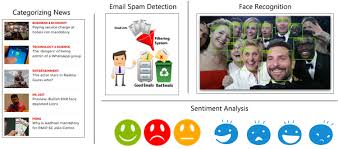
\includegraphics[width=.8\textwidth]{download (1).jpg}
    \caption{Naive Bayes uses a similar method to predict the probability of different class based on various attributes. This algorithm is mostly used in text classification and with problems having multiple classes.}
\end{figure}

\section{Advantages}

It is a relatively simple algorithm to understand and build.
It is faster to predict classes using this algorithm than many other classification algorithms.
It can be easily trained using a small dataset.

\section{Disadvantages}

One of the problems of Naïve Bayes is known as the "Zero Conditional Probability Problem." This problem wipes
out all the information in other probabilities too. There are several sample correction techniques to fix this problem
such as "Laplacian Correction."
Another disadvantage is the very strong assumption of independence class features that it makes. It is near to
impossible to find such data sets in real life.




\section{Conclusions}
This paper presents the review of Naive Bayes Algorithm whichdiscussed enlarged Naïve Bayes text arrangement, Spam filtration, Sentiment investigation, and Recommendation System are a portion of the significant uses of this calculation. It has additionally a few issues, for example, Zero Conditional Probability Problem and how to settle it. The key issue in guileless Bayes model is a class contingent likelihood assessment, and part thickness assessment is a typical path for that. This lessens the issue to the assessment of twofold integrals. For specific piece capacities and likelihood dispersions, the twofold essential can be diagnostically assessed to give a shut structure equation, permitting a productive recipe based calculation. By and large, notwithstanding, the twofold basic can't be improved in shut structures.




\section{Future Enhancements}
In spite of the way that the sweeping freedom suppositions are frequently off base, the innocent Bayes classifier has a few properties that make it shockingly valuable practically speaking. Specifically, the decoupling of the class restrictive component dispersions implies that every appropriation can be autonomously assessed as a one-dimensional circulation. This eases issues coming from the scourge of dimensionality, for example, the requirement for informational indexes that scale exponentially with the quantity of highlights. While guileless Bayes frequently neglects to deliver a decent gauge for the right class probabilities,[17] this may not be a necessity for some applications. For instance, the guileless Bayes classifier will settle on the right MAP choice standard arrangement insofar as the right class is more plausible than some other class. This is genuine whether or not the likelihood gauge is marginally, or even terribly erroneous. Thusly, the general classifier can be powerful enough to overlook genuine inadequacies in its hidden guileless likelihood model.



\begin{thebibliography}{99}

\bibitem{melissinos}
A Novel Bayes Model, Hidden Naive Bayes‖, IEEE Transaction on
Knowledge and Data Engineering, Vol 21, No. 10, pp. 1361 – 1371
\bibitem{melissinos}
Learning the naive Bayes classifier with optimization models,‖ vol. 23, no. 4, pp. 787–795,
2013.
\bibitem{melissinos}
Naive Bayes Classification of Uncertain Data,‖ no.
60703110
\bibitem{melissinos}
Three naive Bayes approaches for discrimination-free classification‖, Data MinKnowl Disk, 2010.
\bibitem{Cyr}
Structured Features in Naive Bayes Classification‖, Association for
the Advancement of Artificial Intelligence, 2016.
\bibitem{melissinos}
Top 10 algorithms in data mining‖, Springer-Verlag London, 2007
\bibitem{Wiki} 
Based on preventing SQL injection network security technology analysis and application, 43-50 2010.06.
\end{thebibliography}


\end{document}


